\documentclass[10pt]{beamer}
\usepackage[utf8]{inputenc}
\usepackage{xeCJK}
\usepackage{graphicx}
\usepackage {mathtools}
\usepackage{utopia} %font utopia imported
\usetheme{CambridgeUS}
\usecolortheme{dolphin}
\usepackage{xcolor}%[dvipsnames]
%\usepackage[hidelinks]{hyperref}
%\usetheme{Copenhagen}
%\newenvironment{vblock}[3]{%
%\setbeamercolor{block body}{#2}
%\setbeamercolor{body title}{#3}
%\begin{block}{#1}}{\end{block}}


% set colors
%\definecolor{myNewColorA}{RGB}{126,12,110}
%\definecolor{myNewColorB}{RGB}{165,85,154}
%\definecolor{myNewColorC}{RGB}{203,158,197}
\definecolor{myNewColorA}{RGB}{242,85,37}
\definecolor{myNewColorB}{RGB}{247,124,40}
\definecolor{myNewColorC}{RGB}{255,209,84}
% \definecolor{myNewColorA}{RGB}{10,85,230}
% \definecolor{myNewColorB}{RGB}{10,124,215}
% \definecolor{myNewColorC}{RGB}{10,209,190}
\setbeamercolor*{palette primary}{bg=myNewColorC}
\setbeamercolor*{palette secondary}{bg=myNewColorB, fg = white}
\setbeamercolor*{palette tertiary}{bg=myNewColorA, fg = white}
\setbeamercolor*{titlelike}{fg=myNewColorA}
\setbeamercolor*{title}{bg=myNewColorA, fg = white}
\setbeamercolor*{item}{fg=myNewColorA}
\setbeamercolor*{caption name}{fg=myNewColorA}
\setbeamercolor*{block title}{use=structure,fg=white,bg=myNewColorB}
\setbeamercolor*{block body}{use=structure,fg=black,bg=myNewColorC}
\usefonttheme{professionalfonts}
\usepackage{natbib}
\usepackage{hyperref}
%------------------------------------------------------------
\titlegraphic{
\includegraphics[height=2.2cm]{9019.jpg}}

\setbeamerfont{title}{size=\large}
\setbeamerfont{subtitle}{size=\small}
\setbeamerfont{author}{size=\small}
\setbeamerfont{date}{size=\small}
\setbeamerfont{group}{size = \small}
\setbeamerfont{institute}{size=\small}
\title{Explaining answers given by neural question answering systems}
\subtitle{AI2100 | Deep Learning}

\author[{Group-35}]{ Pranav(AI20BTECH11004)  \and Chirag (AI20BTECH11006)
\and Dishank(AI20BTECH11011) \and Adhvik(AI20BTECH11015)\and Yashas(AI20BTECH11027)}

\institute{IIT Hyderabad}
\date{\today}

\AtBeginSection[]{
  \begin{frame}
  \vfill
  \centering
  \begin{beamercolorbox}[sep=8pt,center,shadow=true,rounded=true]{title}
    \usebeamerfont{title}\insertsectionhead\par%
  \end{beamercolorbox}
  \vfill
  \end{frame}
}
%------------------------------------------------------------

\begin{document}

%The next statement creates the title page.
\frame{\titlepage}
\begin{frame}
\frametitle{Contents}
\tableofcontents
\end{frame}
\section{Abstract}
\begin{frame}{Abstract}
Question answering has been a fundamental challenge in NLP with vast applications. State of the art neural question answering systems are able to beat humans at this task when evaluated on carefully prepared datasets. However it is difficult to explain in human comprehensible manner, how these models reach the answers that they do. Such an explanation is often important in high stakes situations such as healthcare or business applications. Hence, we explored various explainability methods in the context of neural question answering through this project and verified some of their results. We also report our findings and frame adversarial examples to support our claims.
\end{frame}

\section{Initial Literature Review}
\subsection{Question Answering and Explainable AI}
\begin{frame}{Question Answering}
\begin{itemize}
    \item 
    Question answering (QA):
        \begin{itemize}
            \item It is the task of providing accurate answers to questions posed in natural language.
            \item QA can be broadly studied under two categories: Open domain and Closed domain
            \item \textbf{Closed domain QA}  is provided with a question and a corresponding text which may have the answer to the question.
            \begin{itemize}
                \item  It provides a measure for how well a system understands text. Some popular datasets for this task are SQuAD 1.1 and SQuAD 2.0 datasets
            \end{itemize}
            \item \textbf{Open domain QA} is not provided a corresponding text but has to perform additional information retrieval operations on public knowledge bases like Wikipedia or internet.
            \begin{itemize}
                \item Such QA systems are of importance as they are already being integrated into search engines and voice assistants.
            \end{itemize}
        \end{itemize}
        \end{itemize}
\end{frame}

\subsection{Methods in Question Answering}

\begin{frame}{Methods in Question Answering}
\begin{itemize}
    \item In the early days, the question answering systems such as BASEBALL~\cite{BASEBALL}, SHRDLU~\cite{SHRDLU} were procedural, their knowledge bases were targeted at specific domain, the data needed to be carefully prepared by experts in the domain and they were not resilient to syntactic variations.
    \item Around 1990s RNNs were popular for language inference tasks, but they have their own limitations of vanishing gradient. While, LSTM~\cite{LSTM} maintain constant error propagation, they tend to be computationally inefficient, easy to overfit
    \item Transformer~\cite{Transformer} models build on the model of self-attention, and it introduces multi-head self-attention. This makes transformers parallelizable, and faster. 
    \item BERT which is used in Google search engine is a transformer based model. It is pre-trained on large corpus of data including that from Wikipedia. It can be fine-tuned on small dataset for specific tasks.
\end{itemize}
\end{frame}
\begin{frame}{Explainable AI}
    \begin{itemize}
        \item Explainable AI (XAI) seeks to understand how machine learning models arrive at their predictions. What might consist an explanation is debatable.
        \item XAI systems must follow four principles~\cite{Nist} set out by the National Institute of standards and technology:
\begin{itemize}
    \item \textbf{Explanation}: Systems deliver accompanying evidence or reason(s) for all outputs
    \item \textbf{Meaningful}: Systems provide explanations that are understandable to individual users
    \item \textbf{Explanation Accuracy}: The explanation correctly reflects the system’s process for generating the output 
    \item \textbf{Knowledge Limits}: The system only operates under conditions for which it was designed or when the system reaches a sufficient confidence in its output
\end{itemize}

\item Explanations for machine learning models are important as they greatly help in building trust in the models. Such explanations can also pave the way to build better models in the future.
    \end{itemize}
\end{frame}
\subsection{Methods in Explainable AI}
\begin{frame}{Methods in Explainable AI}
\begin{itemize}
    \item Intrinsic and post hoc explanations, are the two common types of explanations in XAI
    \item Intrinsic explanations rely on the interpretability of the model in use.
    \begin{itemize}
    \item ex: linear models and decision trees are considered inherently explainable. 
    \item Not suited for deep learning models as they are not easily interpretable.
    \end{itemize}
    \item Post hoc explanations try to provide explanations for individual predictions of the model.
    \begin{itemize}
    \item ex: which part of the input was important for getting the output or what representations did the model learn for a particular input. 
    \item Some approaches like LIME ~\cite{lime}, counterfactual examples ~\cite{counterfactual} are model-agnostic.
    \item Approaches like Saliency maps~\cite{Saliency}, Integrated Gradients~\cite{IG} are specific to deep learning models.
    \end{itemize}
\end{itemize}
\end{frame}

\section{Further Literature Review}
\begin{frame}{Further Literature Review}
\begin{itemize}
    \item We focused our further literature review on explainability of BERT for QA.
    \item Although transformers are believed to be moderately interpretable through the inspection of their attention values, ~\cite{at_not_exp} shows that this may not be the case always.
    \item ~\cite{bert_for_qa} attempts to interpret layer-wise functionality in BERT for RCQA using Integrated Gradients.
    \begin{itemize}
        \item They found that the initial layers of BERT focus on query-passage interaction, while 
        \item The later layers focus more on task specific functionalities such as contextual understanding, improving the answer predictions, etc.
    \end{itemize}
\end{itemize}
\end{frame}

\begin{frame}{Further Literature Review Contd.}
\begin{itemize}
    \item ~\cite{bert_layers_qa} proposes that the hidden states contain valuable information that can be leveraged to get interpretable results.
    \begin{itemize}
        \item They applied a set of general and QA specific probing tasks to get an insight into internal representations in transformer layers. 
        \item They also performed visualization of hidden representations, using dimensionality reduction techniques like PCA ~\cite{PCA} to get further insight.
        \item They show that transformations within BERT go through phases that are related to traditional pipeline tasks. 
        \item These phases are also analogous to human reasoning processes.
    \end{itemize}
\end{itemize}
\end{frame}

\section{Implementation}
\begin{frame}{Implementation}
We have used an BERT-base-uncased model from the Hugging face library which is fine-tuned on the SQuAD-v1 to analyse the layer attributions. We used \textbf{Integrated Gradients} from \href{https://captum.ai/}{\textbf{Captum}} (an explainable AI toolkit) to compute the attribution scores for each word.
Integrated Gradients for a model $F$ and input $x_i$ is calculated as follows:
\begin{equation}
    \displaystyle IG(x_i) = \int_{0}^{1}\frac{\partial F(\tilde{x}+\alpha(x_i - \tilde{x} )}{\partial x_i} d\alpha
\end{equation}
\end{frame}
\begin{frame}{Implementation Contd.}
We obtained the following result
\begin{figure}[h]
    \centering
    \onecolumn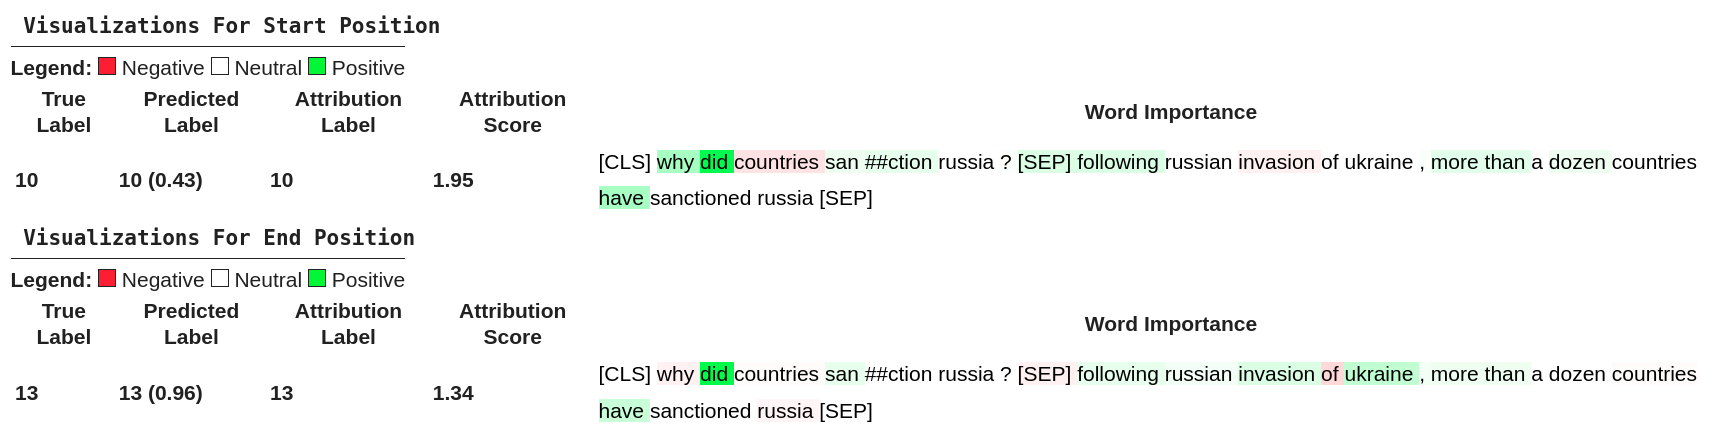
\includegraphics[scale=0.2]{1.png}
    \caption{Visualization of attribution scores for each input word.}
    \label{fig:my_label}
\end{figure}


\centerline{\textbf{Predicted Answer :} russian invasion of ukraine}
\end{frame}



\section{Approach}
\begin{frame}{Approach}
We analysed BERT model for the task of RCQA using integrated gradients. We fine-tuned BERT-base-uncased for 3 epochs on SQuAD-v1 and saved the fine-tuned model. To understand what the fine-tuned BERT is looking at, and to explain the functionality of its layers, we propose to use the embeddings that are produced after each layer. A few previous works look at attention scores produced by BERT to conclude facts about interpretability. But, more recent work \cite{at_not_exp} shows that attention, atleast in some cases, is not suited for explainability.
\end{frame}

\begin{frame}{Approach Contd.}
 Hence we chose to work on the embeddings which carry some information about what BERT has learnt, from each layer. We analyse them using two approaches:
\begin{enumerate}
    \item Visualisations of integrated gradients of embeddings, after each layer
    \item t-SNE visualisations of the embeddings, after each layer.
\end{enumerate}
In the following section, we verify some of the results which previous works have found. Also, we outline our findings for the fine-tuned model.
\begin{enumerate}
    \item Using Integrated gradient technique, we came to the conclusion that Bert model uses certain heuristics to answer question.
    \item To further verify this claim, we built adversarial examples on which these heuristics would not work. We found that Bert model did fail on these adversarial examples.
\end{enumerate}
\end{frame}

\section{Results}
\subsection{Verification of some of the previous works} \label{section2.1}
\begin{frame}{Verification of some of the previous works}
\begin{enumerate}
    \item \cite{bert_for_qa} claims that initial layers of BERT focus on words common to the question and the passage. In the later layers, the focus on such words decreases, and more focus is on supporting words that surround the answer. Their approach uses Integrated Gradients. Proceeding on similar lines, we confirm their claims.
\end{enumerate}

We calculated the attribution scores for embeddings of words after each layer using integrated gradients approach. We leveraged the captum library to achieve this. We visualised these using the inbuilt-captum functionality, as well as by plotting the heatmaps. We indeed get similar results \ref{fig:plot1} which the paper claims. Initial layers focus more on words common to the question and the context. Later layers, try to look at supporting context words. Finally, the model focuses on the answer in the last layers.
\end{frame}

\begin{frame}{Verification Contd.}
Consider the context-question pair given below.\\
\textbf{Context: }The Panthers finished the regular season with a 15–1 record, and quarterback Cam Newton was named the NFL Most Valuable Player (MVP). They defeated the Arizona Cardinals 49–15 in the NFC Championship Game and advanced to their second Super Bowl appearance since the franchise was founded in 1995. The Broncos finished the regular season with a 12–4 record, and denied the New England Patriots a chance to defend their title from Super Bowl XLIX by defeating them 20–18 in the AFC Championship Game. They joined the Patriots, Dallas Cowboys, and Pittsburgh Steelers as one of four teams that have made eight appearances in the Super Bowl. The 2020 regular season win/loss ratio for the Michigan Vikings was 656.\\
\textbf{Question: }How many appearances have the Broncos made in the super bowl?\\
\textbf{Predicted Answer: }eight\\
\end{frame}
\begin{frame}{Verification Contd.}
    \begin{figure}
    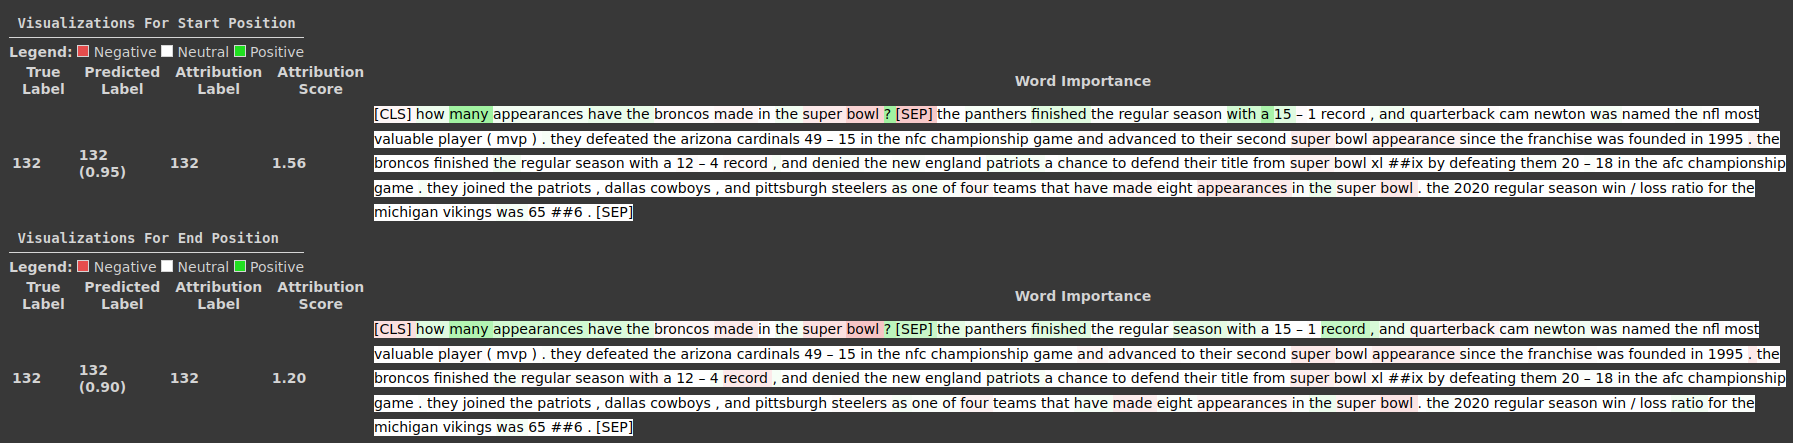
\includegraphics[width=\linewidth]{ll0.png}
    \caption{Visualisation of Integrated gradients of word embedding after layer 0.}
    \label{fig:plot1}
\end{figure}
\end{frame}

\begin{frame}{Verification Contd.}
\begin{figure}
    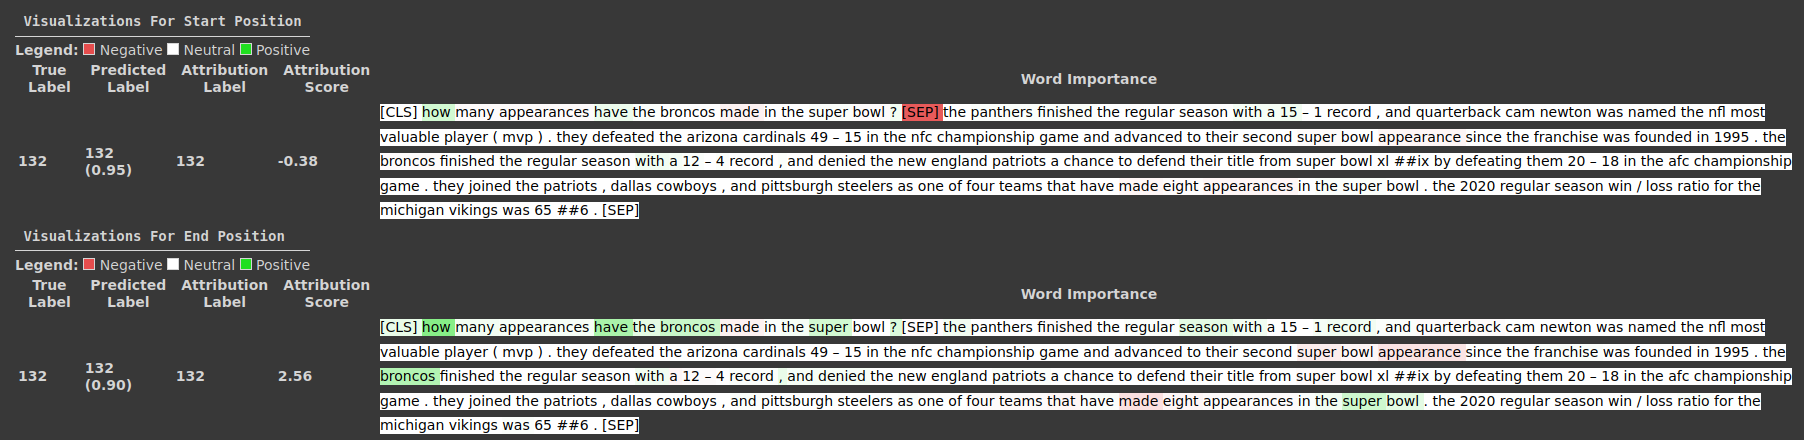
\includegraphics[width=\linewidth]{ll1.png}
    \caption{Visualisation of Integrated gradients of word embedding after layer 3.}
\end{figure}
\end{frame}

\begin{frame}{Verification Contd.}
\begin{figure}
    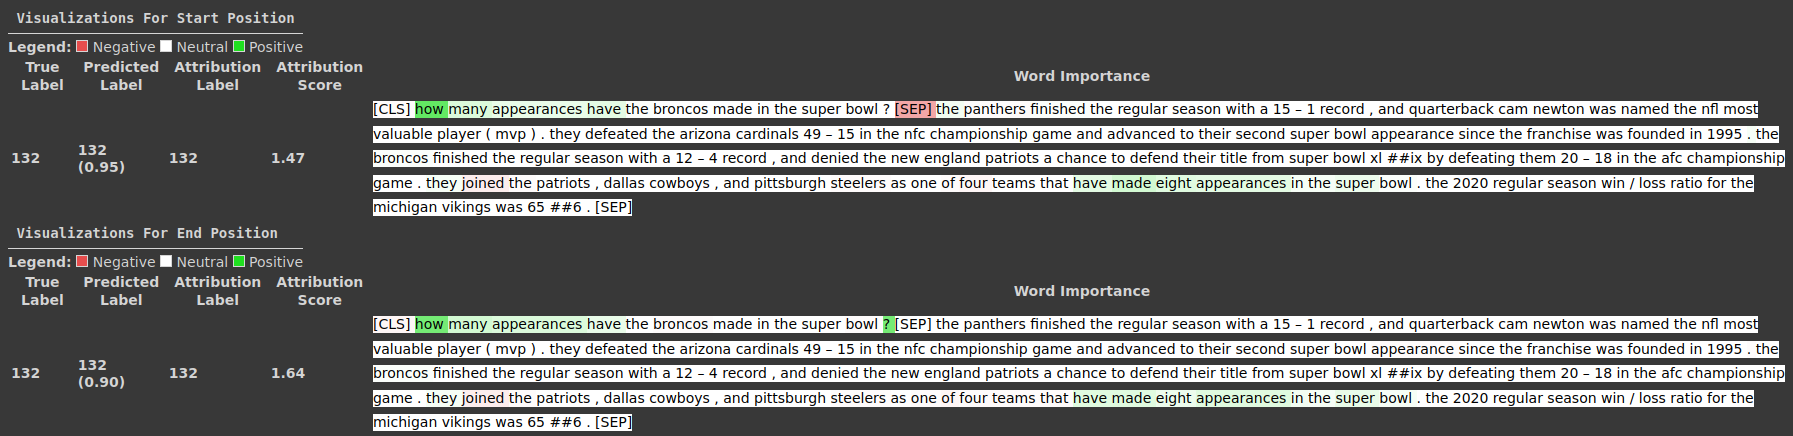
\includegraphics[width=\linewidth]{ll5.png}
    \caption{Visualisation of Integrated gradients of word embedding after layer 7.}
\end{figure}
\end{frame}

\begin{frame}{Verification Contd.}
\begin{figure}
    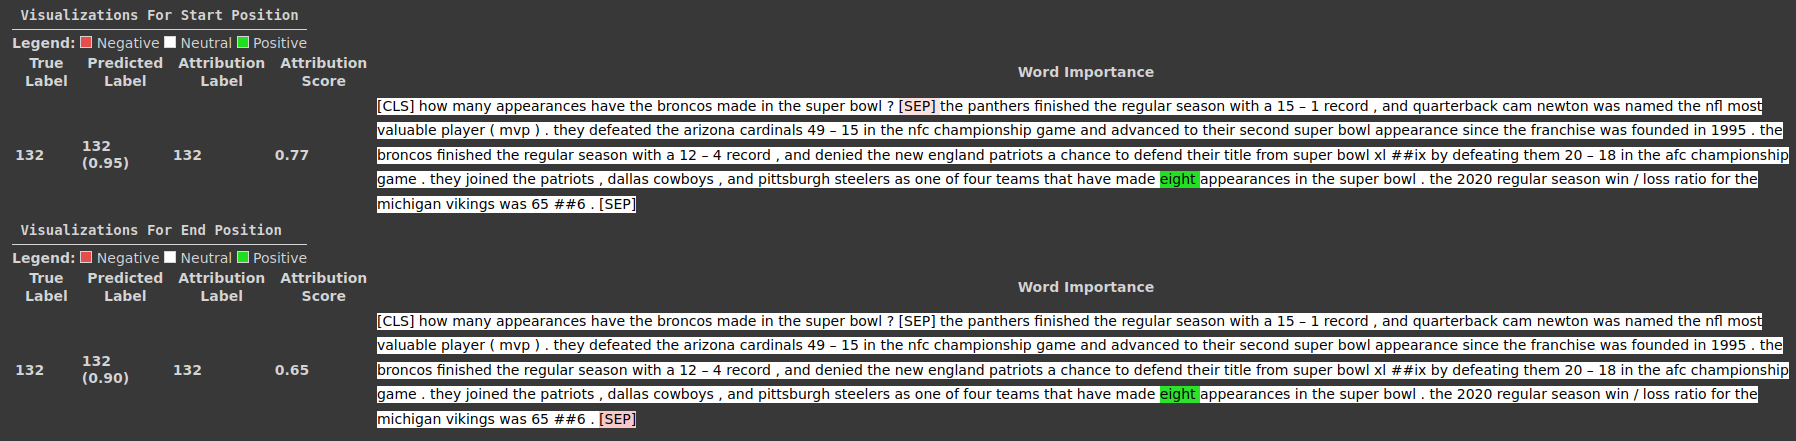
\includegraphics[width=\linewidth]{ll11.png}
    \caption{Visualisation of Integrated gradients of word embedding after layer 11.}
\end{figure}
\end{frame}
\begin{frame}{Verification Contd.}

\begin{enumerate}[2]
    \item \cite{bert_layers_qa} claims that initial layers look at the semantic meanings of each word, and subsequent layers look at relations between the words in context. The final layers filter out the relevant information, and come up with the answer. Their approach uses PCA visualisation of embeddings.  Proceeding on similar lines, we confirm their claims.
\end{enumerate}
We perform t-SNE visualisations of embeddings after each layer, instead of PCA, in order to preserve more information, which might have possibly lost during PCA. We indeed get similar results \ref{fig:plot2} which the paper claims. Initial layers look at semantic meanings of words (words like white, black or loves, like, or cat, dog occur together). Later layers, learn relations in context (white, cat, black, dog become together). Finally, all the important information is filtered out (apples, is reasonably seperated).
\end{frame}

\begin{frame}{Verification Contd.}
Consider the context-question pair given below.\\
\textbf{Context: }Alfred is a white cat and likes apples. Bobby is a black dog which loves mangoes.\\
\textbf{Question: }What does Alfred like?\\
\textbf{Predicted Answer: }Apples
\end{frame}

\begin{frame}{Verification Contd.}
\begin{figure}
    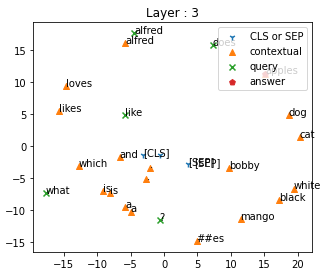
\includegraphics[scale = 0.5]{layer_3.png}
    \caption{t-SNE visualisations of word embeddings after layer 3.}
    \label{fig:plot2}
\end{figure}
\end{frame}

\begin{frame}{Verification Contd.}
\begin{figure}
    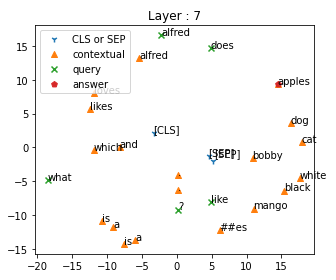
\includegraphics[scale=0.5]{layer_7.png}
    \caption{t-SNE visualisations of word embeddings after layer 7.}
\end{figure}
\end{frame}

\begin{frame}{Verification Contd.}
\begin{figure}
    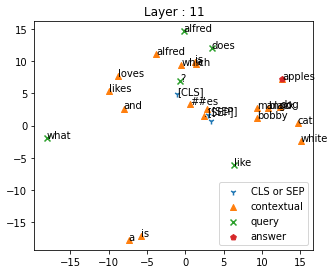
\includegraphics[scale=0.5]{layer_11.png}
    \caption{t-SNE visualisations of word embeddings after layer 11.}
\end{figure}
\end{frame}

% \begin{frame}{Verification Contd.}
 
% \end{frame}

\subsection{Some of our (interesting) findings}
\begin{frame}{Some of our (interesting) findings}
Analysing the heat-maps for different examples, we observed few patterns. First was that initially the model was focusing greatly on question words like "Who, What, When, Where". The model was also focusing on possible answers to such nouns and numbers in the query.
\\
Consider the context-question pair given below \ref{ex1}\\
\textbf{Context: }93 players have been awarded the Fewest Prized Team distinction for the Champ Bowl.\\
\textbf{Question: }How many players have been awarded the Fewest Prized Team distinction for the Super Bowl?\\
Second was that as mentioned previously, the model was focusing on words which were same in the question and the context. Then the model was looking at neighbours of the words it focused on initially, as mentioned above. (Look at section \ref{section2.1}).
\end{frame}

\begin{frame}{Verification Contd.}
\begin{figure}
    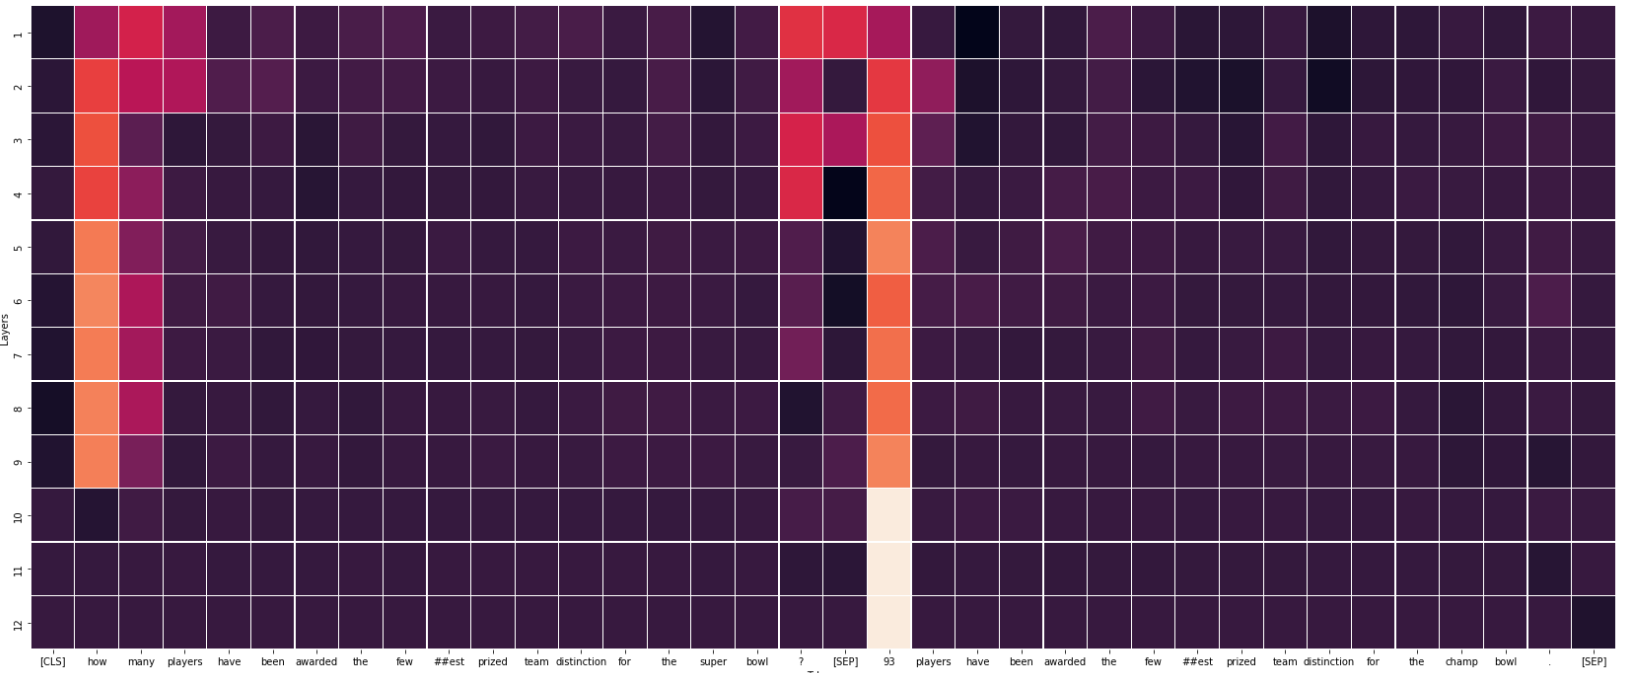
\includegraphics[scale=0.2]{obs1.png}
    \caption{Example demonstrating importance in initial layers}
    \label{ex1}
\end{figure}
\end{frame}

\begin{frame}{Findings contd.}
    Based on these observations, we claim that the Bert model uses heuristics to predict the start and end tokens. These heuristics work as follows:

\begin{enumerate}
    \item Recognize the question type by focusing on the question words. Focus on candidate answers.
    \item Focus on words that are same in both the question and the answer.
    \item Look at neighbouring words of the words on which we focused in the above steps and predict start and end tokens from these.
\end{enumerate}

How exactly the model picks start and end token during heuristic 3 is still a mystery.
\end{frame}

\subsection{Verification of the claims using adversarial examples}
\begin{frame}{Verification of the claims using adversarial examples}
We constructed adversarial examples by assuming that the model uses these heuristics. We expected that the model to fail on these examples and that is exactly what happened.

To test heuristic 1, consider the context-question pair given below\\
\textbf{Context: }Yes, a person can jump from a hill and still be alive.\\
\textbf{Question: }After jumping from a hill, can a person be alive?\\
\textbf{Predicted Answer: }still be alive 
\end{frame}



\begin{frame}{Verification Contd.}
Clearly, the model fails here. To test heuristic 2, we constructed examples where there were no similar words or where there were more than one similar word.

Consider the context-question pairs given below 

\textbf{Context: }Trump has a Trump card having his photo.

\textbf{Question: }What has Trump's photo?

\textbf{Predicted Answer: }Trump has a Trump card

\textbf{Context: }Ram was drawing with pencils. Teacher was picking her nose with pencil. Ram observed that pencils can be used to pick nose.

\textbf{Question: }What was Ram's conclusion?

\textbf{Predicted Answer: }None
\end{frame}

\begin{frame}{Verification Contd.}
In the last example, if "conclusion" is replaced with "observation" in the query, the model gives correct output. This further shows the necessity of same words. This also makes the model brittle and easy to fool because there is a lack of language understanding.
\end{frame}

\begin{frame}{Verification Contd.}
To test heuristic 3, we constructed an example in which the correct answer was much farther than words on which model is focusing using heuristic one and two.
Consider the context-question pair given below \ref{obs2}\\
\textbf{Context: } Ram had a big white great beautiful majestic creative cute cat and bad dog.\\
\textbf{Question: } What did Ram have that was bad?\\
\textbf{Predicted Answer: } a big white great beautiful majestic creative cute cat and bad dog \\
\end{frame}
\begin{frame}{Verification Contd.}
\begin{figure}
    \centering
    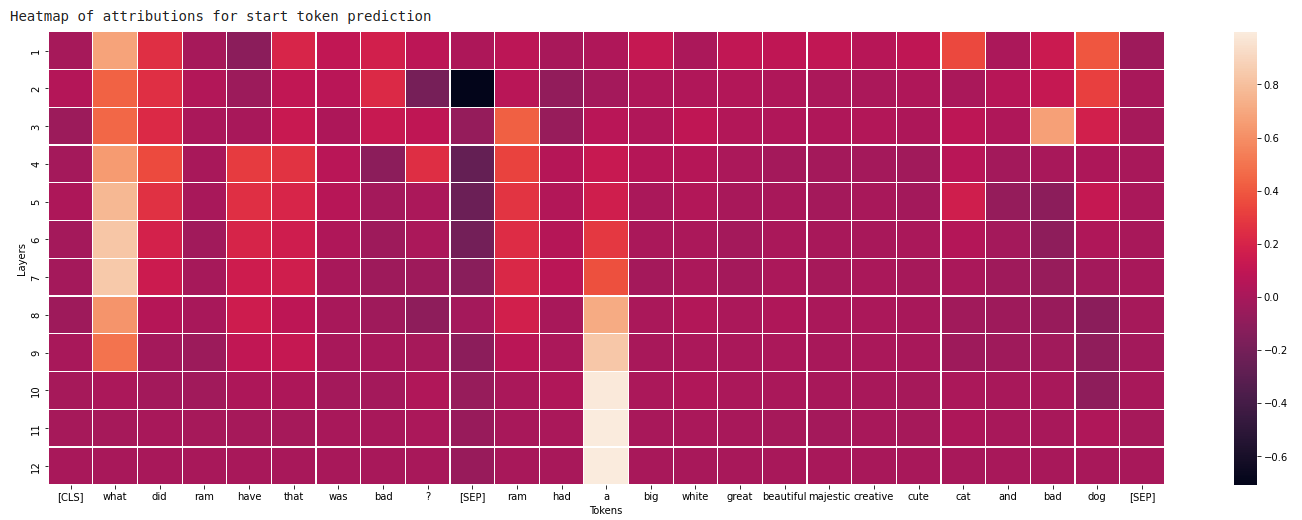
\includegraphics[scale=0.25]{Screenshot from 2022-05-02 20-32-03.png}
    \caption{Adversarial example}
    \label{obs2}
\end{figure}
\end{frame}
\begin{frame}{Verification Contd.}
The heat-map for the last example shows us the full story of how the model predicts the answer. First the model focuses on "cat" and "dog" as they are candidate answers for the question word "what". The model also focuses on the word "what". Then the model finds the word "Ram" to be same in both the question and the context. Thus it focuses on "Ram" in the context. Then it looks at it's neighbouring word: "a" and predicts it for start token. The model also focuses on the word "bad" as it is also same in context and question. However, in step 3 of the heuristics, the model chooses to not "go ahead" with the word "bad". 
\end{frame}

\section{References}
\begin{frame}[allowframebreaks]
\bibliographystyle{plain}
\bibliography{egbib} 
\end{frame}

\begin{frame}
\textcolor{myNewColorA}{\Huge{\centerline{\textbf{Thank you!}}}}
\end{frame}

\end{document}



